\documentclass{beamer}
\usepackage[latin1]{inputenc}
\usepackage{tikz}
\usepackage{makecell}
\usepackage{pgfplots}
\usepackage{pgfplotstable} 
%\pgfplotsset{compat=1.12}
\usepackage{sansmath}
\usetheme{Berlin}
\usetikzlibrary{
	arrows.meta,
	chains,
	decorations.pathreplacing,
	automata,
	positioning,
	scopes,
	quotes,
	shapes,
	shadows	
}
\title{Fast Decompression Lucene Codec}
\author{Ivan Mamontov\\ Grid Dynamics}
\institute{Berlin Buzzwords}
\date{Jun 1st, 2015}
\titlegraphic{
	
\includegraphics[width=3.8cm]{resources/buzzwordslogo.png}			\hspace*{8.75cm}~
}


\pgfplotstableread[col sep=comma]{
a,b,c,d,e
128,  82.638  ,200.452 ,194.441  ,330.123  
256,  139.914 ,261.881 ,346.855  ,583.440  
512,  225.505 ,341.506 ,592.312  ,1046.636 
1024, 396.605 ,518.709 ,1100.371 ,2149.478 
2048, 743.370 ,868.560 ,2089.506 ,4058.115 
4096, 1436.633,1557.861,4204.929 ,8023.846 
8192, 2827.855,2953.913,7758.365 ,14458.539
16384,5654.820,5779.984,14938.887,25235.819
}\mytable

\begin{document}
	\begin{frame}
		\titlepage
	\end{frame}
	\begin{frame}
    		\begin{itemize}
    		    \item TOC!!!
		\end{itemize}
  	\end{frame}
  	\begin{frame}
  		\frametitle{Data encoding and file formats}
  		\begin{itemize}
  			\item Lucene 3.x and before
  			\begin{itemize}
  				\item Tuned to pre-defined data types
  				\item Combinations of delta encoding and variable length byte encodings
  				\item Hardcoded choices -- impossible to customize
  				\item Dependencies on specific file-system behaviors
  				\item Data coding happened in many places
  			\end{itemize}
	  			\item Lucene 4 and onwards
  					\begin{itemize}
  						\item All data writing and reading abstracted from data encoding
  						\item Highly customizable, easy to use API
  					\end{itemize}		
  		\end{itemize}
  	\end{frame}
  	\begin{frame}
  		\frametitle{Lucene 5.0 index format}
  		The default Lucene50 codec is:
  		\begin{itemize}
  			\item variable-byte and fixed-width encoding of delta values
  			\item multi-level skip lists
  			\item natural ordering of docIDs
  			\item encodes both term frequencies and positional information
  		\end{itemize}
  	\end{frame}

  	\begin{frame}
  		\frametitle{What is variable-byte encoding?}
%  		\begin{itemize}
%  			\item uses an integral number of bytes to encode a gap
%  			\begin{itemize}
%  				\item the first bit of the byte is a continuation bit. It is set to 1 for the last byte of the encoded gap and to 0 otherwise
%  				\item the last 7 bits of a byte are \textbf{payload} and encode part of the gap
%  			\end{itemize}
%  		\end{itemize}
  		Encode sequence of numbers into variable-length bytes using one status bit per byte indicating whether the current number expands into next byte.
  	\end{frame}
  	\begin{frame}
  		\frametitle{What is variable-byte encoding?}
  		To encode the decimal number 6917:
		\vskip15pt 
  		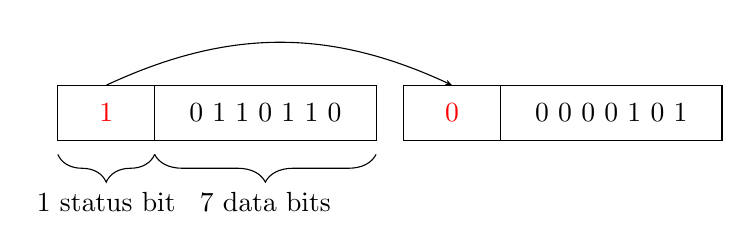
\begin{tikzpicture}[
 		      	start chain = going right,
     			node distance = 0pt,
				ArrayStyle/.style={draw, minimum width=3.5em, minimum 									height=2em, outer sep=0pt, on chain}]
			\node [ArrayStyle] (1) {{\color{red!100}1}};
			\node [ArrayStyle, minimum width=8em] (2) {0 1 1 0 1 1 0};
			\node [ArrayStyle, xshift=1em] (3) {{\color{red!100}0}};
			\node [ArrayStyle, minimum width=8em] (4) {0 0 0 0 1 0 1};
			\begin{scope}[-{Stealth[length = 2.5pt]}]
  				\draw (1.north) [out=25, in=155] to (3.north);
			\end{scope}
			\draw[decorate,decoration={brace, amplitude=10pt, 					raise=5pt, mirror}]
  				(2.south west) to node[black,midway,below= 15pt] 				{$7$ data bits} (2.south east);
			\draw[decorate,decoration={brace, amplitude=10pt, 					raise=5pt, mirror}]
  				(1.south west) to node[black,midway,below= 15pt] 				{$1$ status bit} (1.south east);
		\end{tikzpicture} 
		\vskip15pt 	
		\pause
		Thus needs 2 bytes instead of 4 bytes!
  	\end{frame}
  	\begin{frame}
  		\frametitle{What is variable-byte encoding?}
  		\begin{itemize}
    		    \item pros
    		    \begin{itemize}
    		    		\item wonderfully simple
    		    		\item good compression rate
    		    \end{itemize}
    		    \item cons
    		    \begin{itemize}
    		    		\item it requires an if statement on every byte	during decode, which is very costly since the CPU cannot easily predict the branch outcome.
    		    \end{itemize}
		\end{itemize}
  	\end{frame}
  	\begin{frame}
  		\frametitle{What is FOR encoding?}
  		Frame-of-reference encoding takes each fixed block of integers and stores them all as packed values, where each value gets N bits, set by the maximum int in the block.	
  	\end{frame}
  	\begin{frame}
  		\frametitle{What is FOR encoding?}
  		To encode the following numbers 1, 3, 7, 10, 13, 14, 18:
		\vskip15pt 
  		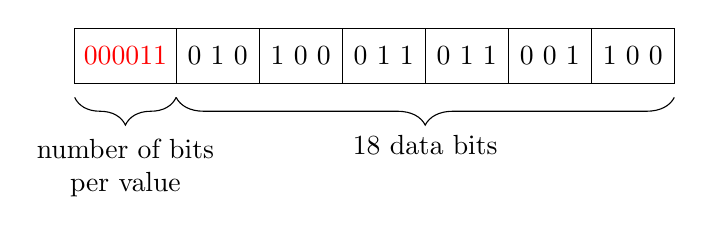
\begin{tikzpicture}[
 		      	start chain = going right,
     			node distance = 0pt,
				ArrayStyle/.style={draw, minimum width=3.5em, minimum 									height=2em, outer sep=0pt, on chain}]		
			\node [ArrayStyle] (1) {{\color{red!100}000011}};
			\node [ArrayStyle, minimum width=3em] (2) {0 1 0};
			\node [ArrayStyle, minimum width=3em] (3) {1 0 0};
			\node [ArrayStyle, minimum width=3em] (4) {0 1 1};
			\node [ArrayStyle, minimum width=3em] (5) {0 1 1};	
			\node [ArrayStyle, minimum width=3em] (6) {0 0 1};
			\node [ArrayStyle, minimum width=3em] (7) {1 0 0};	
			\draw[decorate,decoration={brace, amplitude=10pt, 					raise=5pt, mirror}]
  				(2.south west) to node[black,midway,below= 15pt] 				{18 data bits} (7.south east);
			\draw[decorate,decoration={brace, amplitude=10pt, 					raise=5pt, mirror}]
  				(1.south west) to node[black,midway,below= 15pt] 				{\makecell[c]{number of bits\\per value}} (1.south east);
		\end{tikzpicture} 
		\vskip15pt 	
		\pause
		Thus needs 3 bytes instead of $7*4=32$ bytes!
  	\end{frame}
  	\begin{frame}
  		\frametitle{What is FOR encoding?}
  		\begin{itemize}
    		    \item pros
    		    \begin{itemize}
    		    		\item two times faster during decoding than VInt % Up to 2 times faster than in \mbox{variable-byte} encoding
    		    		\item {\color{red!100} TODO something about SIMD/modern CPUs}
    		    \end{itemize}
    		    \item cons
    		    \begin{itemize}
    		    		\item in order to access even one int within the block, we must decode the full block
    		    		\item requires integers in batches of multiples of 32
    		    \end{itemize}
		\end{itemize}  		
  	\end{frame}
  	\begin{frame}
%With conventional scalar operations, four add instructions must be executed one after another to obtain the sums as shown
    		\frametitle{What is SISD?}
    		Single Instruction Single Data (SISD)
    		\vskip15pt 
  		\tikzset{% define the style of the nodes for drawing the squares
     		mysquare/.style={shape=rectangle,draw=black!                       			100,thick,top color=white}
   		}

  		\begin{tikzpicture}
    			\foreach \x in {0,...,3} {% loop over the three rows
       		\node[mysquare] at (0,-\x) {$A_\x$};
       		\node at (1,-\x) {$+$};
       		\node[mysquare] at (2,-\x) {$B_\x$};
       		\node at (3,-\x) {$=$};
       		\node[mysquare] at (4,-\x) {$C_\x$};
    			}
		 \end{tikzpicture}
		
  	\end{frame}
  	\begin{frame}
    		\frametitle{What is SIMD?}
    		\begin{itemize}
    		    \item Single Instruction Multiple Data (SIMD)
    		    \vskip15pt 
  			\tikzset{
     			mysquare/.style={shape=rectangle,draw=black!			                100,thick,top color=white}
   			}
		    \begin{tikzpicture}% use positioning to put the boxes together
    				\foreach \letter/\col/\x in {A/yellow!30/0, B/green!40/2, C/red!50/4} {
      				\node[mysquare=\col] (\letter 0) at (\x,0){$\letter_0$};
      				\node[below=-1pt of \letter 0,mysquare=\col] (\letter 1) {$\letter_1$};
      				\node[below=-1pt of \letter 1,mysquare=\col] (\letter 2) {$\letter_2$};
      				\node[below=-1pt of \letter 2,mysquare=\col] (\letter 3) {$\letter_3$};
    				}
    				\node at (1,-0.8) {$+$};% place + and = by hand
    				\node at (3,-0.8) {$=$};
  			\end{tikzpicture}
		\end{itemize}
  	\end{frame}
  	\begin{frame}
    		\frametitle{Why does it matter?}
    		\begin{itemize}
    		    \item pros
    		    \begin{itemize}
    		    		\item 75\% fewer loads
    		    		\item 75\% fewer adds
    		    		\item 75\% fewer stores
    		    \end{itemize}
    		    \item cons
    		    \begin{itemize}
    		    		\item not all algorithms can be vectorized
    		    		\item {\color{red!100}TODO}
    		    \end{itemize}
		\end{itemize}
  	\end{frame}  	
  	\begin{frame}
  		\frametitle{SIMD auto-vectorization in HotSpot}
  		%Sometimes it is possible to move the kernel to C/C++, use SIMD there and call via JNI. However, the cost of the JNI call can be significant as are the difficulties of ensuring memory is properly aligned for SIMD execution
  		%In HotSpot versions beginning with Java 7u40, the server compiler provides support for auto-vectorisation. According to JDK-6340864
		%However, this seems to be true only for "simple loops" - at least for the moment. For example, accumulating an array cannot be vectorised yet JDK-7192383
		Vector arithmetic is not supported yet. Only array initialization and array copy.
  		\begin{itemize}
  			\item \url{http://bugs.java.com/view_bug.do?bug_id=6340864}
  			\item \url{http://bugs.java.com/view_bug.do?bug_id=7192383}
  		\end{itemize}
  	\end{frame}
  	\begin{frame}
  		\frametitle{Cost of JNI Call	in HotSpot}
  		\begin{itemize}
  			\item Move arguments according to ABI.
  			\item Wrap object references to JNI handles.
  			\item Obtain JNIEnv*, jclass/jobject and pass them as parameters.
  			\item Check if should call method\_entry trace function.
  			\item Lock an object monitor if the method is synchronized.
  			\item Check if the native function is linked already.%Function lookup and linking is performed lazily.
  			\item Switch thread from in\_java to in\_native state.
  			\item \textbf{Call the native function.}
  			\item Check if safepoint is needed.
  			\item Return thread to in\_java state.
  			\item Unlock monitor if locked.
  			\item Notify method\_exit.
  			\item Unwrap object result and reset JNI handles block.
  			\item Handle JNI exceptions.
  		\end{itemize}
  	\end{frame}
  	\begin{frame}
  		\frametitle{JDK-7013347 Critical Native}
  		\begin{itemize}
  			\item Critical native looks like JNI method
  			\item Uses \textit{JavaCritical\_} prefix instead of \textit{Java\_}
  			\item JavaCritical interface does not wrap objects
  			\item See details in \url{https://bugs.openjdk.java.net/browse/JDK-7013347}
  		\end{itemize}
  	\end{frame}
  	\begin{frame}
  		\frametitle{JDK-7013347 Critical Native}
  		Critical method should:	
  		\begin{itemize}
  			\item be static and not synchronized
  			\item not throw exceptions
  			\item use java primitives and arrays of primitives
  			\item have "deafult" JNI implementation
  			\item work as fast as possible(it blocks GC)
  		\end{itemize}
  	\end{frame}  
  	\begin{frame}
  		\frametitle{Experiment}
  			%The vectorized version is roughly twice as fast as the scalar version
			\begin{tikzpicture}
			\pgfkeys{/pgf/number format/.cd,use comma,1000 sep={},}
    			\begin{loglogaxis}[
            		log basis x=2,log basis y=2,
            		%label style={font=\tiny},
            		xlabel={Block size},ylabel={Decoding latency, ns/op},
            		legend entries={Critical, JNI, FOR, VInt},
            		xmin=96,xmax=24576,
            		ymin=60,ymax=30720,
            		separate axis lines,
            		axis x line*=bottom,
            		axis y line*=left,
            		axis line style={draw=gray!50},
            	ytick={60,120,240,480,960,1920,3840,7680,15360,30720},           			xtick={96,192,384,768,1536,3072,6144,12288, 24576},
            		yticklabel={\pgfkeys{/pgf/fpu}\pgfmathparse{60*(2^(\ticknum))}%
                        \pgfmathprintnumber[fixed,precision=0]\pgfmathresult%
                        \pgfkeys{/pgf/fpu=false}%
                        },
		            xticklabel={\pgfkeys{/pgf/fpu}\pgfmathparse{2^(7+\ticknum)}%
                        \pgfmathprintnumber[fixed]\pgfmathresult%
                        \pgfkeys{/pgf/fpu=false}%
                        },
            x tick label as interval,
            ymajorgrids,
            tick align=outside,
            legend style={draw=none,fill=none,
                          at={(axis description cs:1.1,0.5)}, 
                          anchor=west,
                          %nodes={font=\tiny}
                          },
            tick label style={font=\tiny}
        ]
        			\addplot[red,very thick,mark=square*]     table[x=a,y=b] {\mytable};    
        			\addplot[green,very thick,mark=triangle*] table[x=a,y=c] {\mytable};    
        			\addplot[blue,very thick,mark=diamond*]   table[x=a,y=d] {\mytable}; 
        			\addplot[orange,very thick,mark=*]        table[x=a,y=e] {\mytable}; 
    			\end{loglogaxis}
		\end{tikzpicture}
	\end{frame}  		
	\begin{frame}
		\frametitle{SIMD codec}
		\begin{itemize}
		    \item based on Lucene50 codec
			\item still in progress so it does not support
			\begin{itemize}
				\item freqs
				\item positions
				\item offsets
				\item payloads
			\end{itemize}			
		\end{itemize}
		Fork me on GitHub \url{http://git.io/vkY1o}
	\end{frame}
	\begin{frame}
		\frametitle{Lucene benchmark}
		\begin{itemize}
			\item indexes all of Wikipedia's English XML export
				\begin{itemize}
					\item only documents are indexed: term frequencies and positions are omitted
					\item one large segment is used(about 1GB)
				\end{itemize}
			\item measures how long it takes to search top 100K frequent terms
			\item environment
			\begin{itemize}
				\item i5-4300M CPU @ 2.60GHz (Haswell)
				\item fedora 21 (kernel 3.17.4)
				\item JRE 1.8.0\_401
				\item gcc 4.9.2 
			\end{itemize}
		\end{itemize}
	\end{frame}
	\begin{frame}
		\frametitle{Benchmarking Results}
		\begin{center}
 			\begin{tabular}{|l|c c c|} 
 				\hline
 				& Lucene50 & SIMD SSE4.1 & SIMD AVX \\ [0.5ex] 
 				\hline
				Indexation & & & \\ 
				Duration s. & 6 & 87837 & 787 \\
 				\hline
 				Search & 7 & 78 & 5415 \\
 				\hline
			\end{tabular}
		\end{center}	
	\end{frame}
	\begin{frame}
		\frametitle{Future work}
	\end{frame}
	\begin{frame}
		\frametitle{Conclusions}
	\end{frame}
\end{document}